\documentclass[a4paper, 12pt]{article}
\usepackage{comment} % enables the use of multi-line comments (\ifx \fi) 
\usepackage{lipsum} %This package just generates Lorem Ipsum filler text. 
\usepackage{fullpage} % changes the margin
\usepackage{cite}
\usepackage{graphicx}
\usepackage{wrapfig}
\usepackage{amsfonts}
\usepackage{float}
\linespread{1.15}
\graphicspath{ {images/} }


\begin{document}
%Header-Make sure you update this information!!!!
\noindent
\large\textbf{Carbon Storage Project} \hfill \textbf{Joshua Zweig} \\
\normalsize Carbon Storage \\
Prof. Lackner \hfill Spring 2016 \\

\begin{centering}
\textbf{Short Listing Saline Reservoirs for Potential Carbon Storage} \\
A Look at the Viability of Candidate Reservoirs in the United States through\\
Fuzzy c-Means Clustering\\
\end{centering}


\section*{Abstract}


\section{Introduction}
\subsection{Carbon Storage}
Scope to US bc available data


Motivation and whats what

\subsection{Potential Storage Site: Saline Formations}

\begin{wrapfigure}{r}{0.5\textwidth} %this figure will be at the right
    \centering
    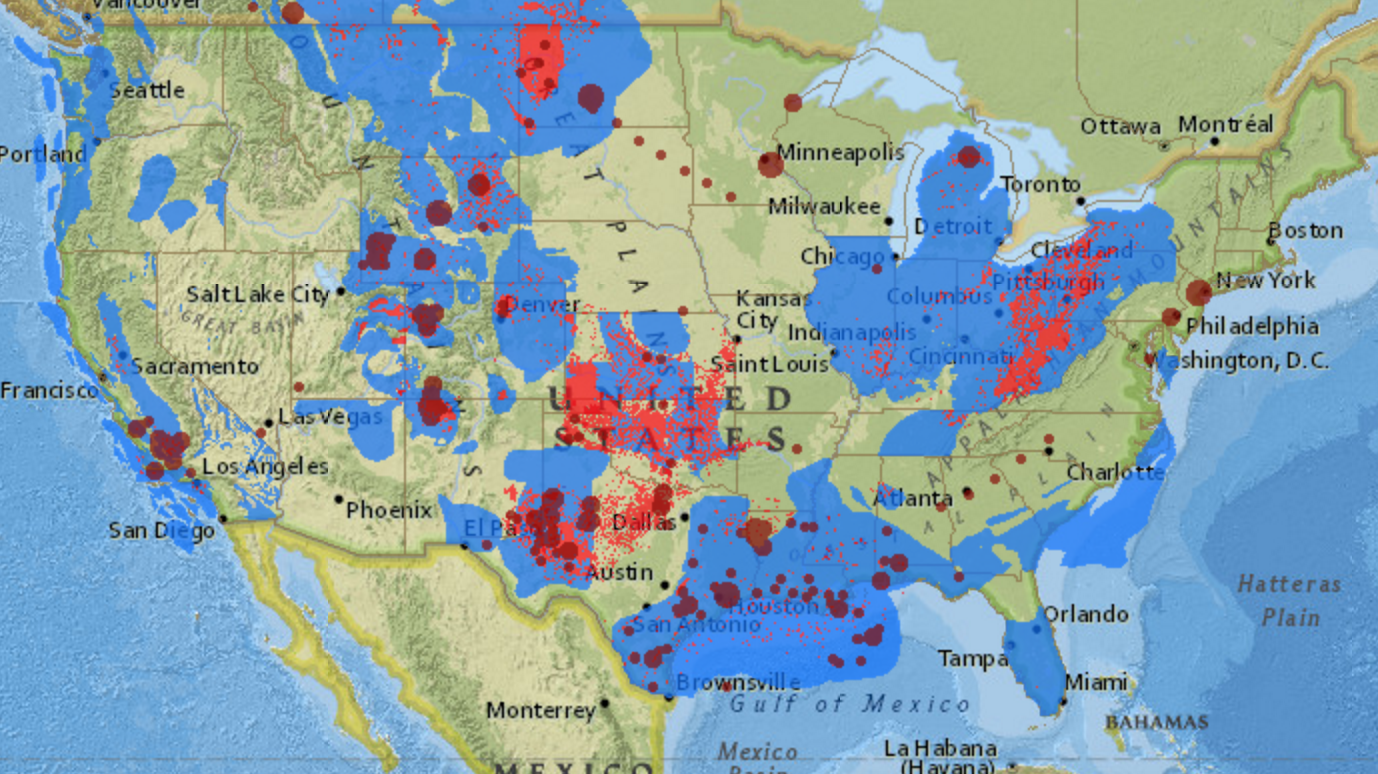
\includegraphics[width=0.5\textwidth]{saline_tight}
    \caption{\label{salinetight} A map of the United States overlaid with geological saline resources for potential carbon storage (blue), stationary sources of petroleum and natural gas (brown) and other oil and gas resources (red) \cite{atlas}}. 
\end{wrapfigure}

\par Of possible candidates for long term carbon sequestration, saline formations have emerged as a promising candidate. Such formations are prevalent throughout North America. These brine coated layers of permeable rock are able to store carbon my way of "solubility trapping, mineral trapping, structural trapping and residual trapping."

The more than 180,000 potential injection sites in the United States have been estimated by the U.S. Department of Energy to have capacity of over 12 trillion tons of CO$_2$. Saline formations are promising also because of their proximity to CO$_2$ point sources, allowing easy transition of U.S. energy assets to "near-zero carbon emissions via low-cost carbon storage retrofits." \cite{whysaline} Furthermore, there is much existing technology and regulatory acceptance with respect to injections into saline reservoirs as brines are frequently injected into saline reservoirs in EOR and the U.S. EPA has designated some deep saline formations for hazardous waste disposal.

\par There are currently at least 3 saline aquifer injection projects that have been undertaken in the continental United States, which have together injected over a million tons of CO$_2$ to date. Each of these projects operates on a time scale of at least twenty years, allocating at least 10 years to "characterizing geologic and terrestrial opportunities for carbon storage and identifying CO$_2$ stationary sources within the territories of the individual RCSPs and evaluating promising CO$_2$ storage opportunities through a series of small-scale field projects"  \cite{midwestinject}, \cite{midwestinject2}, \cite{southeastinject}. 

Important Charecterists 



\subsubsection{Associated Risk} 


\section{Methodology}
\subsection{Overview}
As described in the previous section, saline aquifers are luckily a far vast enough resource for us to currently store the desired amount of carbon. However, selecting the best aquifers for storage is a tremendous task considering the quantity of potential aquifers ($\approx180,000$) and the factors that characterize each one. For this reason we seek to develop a tool to immediately help identify some of the best candidate deep saline aquifers in the United States. 
The fundamental workings of this tool will be in the characterization of potential aquifers based on a series of characteristics as per section \ref{wellchar}. Having fully characterized each candidate aquifer, we fully employ a Fuzzy c-Means clustering analysis to each of the $\approx180,000$, 12 dimensional vectors representing the system to create a model that will determine how strongly each aquifer is characterized by each of the 12 features, to be discusses further in section \ref{fuzz}. Once this model is created, it will allow researchers to essentially filter potential storage sites by different characteristics. For example, we will be able to observe all aquifers that have at least a given storage capacity and/or are at least a given distance from a major fault line.  

\subsection{Saline Aquifer Characterization} \label{wellchar}
Each of the 12 characterization features falls into one of two categories. The first category of features describes the geological aspects of the aquifer, strictly its ability to store carbon. The second describes some of the factors that effect the potential risks and barriers to societal acceptance regarding potential storage sights. 

\subsubsection{Geological Characterization}
Natcarb

\subsubsection{non-Geological Characterization}

The list below is a list of dimensions used to characterize saline formations with respect to environmental features not directly related to the ability of the formation to store carbon.
They are listed with reasonings for their inclusion in this early stage work in no particular order. 


\begin{enumerate}
\item \emph{Potential Impact on Drinking Water Sources} It comes as no surprise that the proximity of a potential injection site to an important source of drinking water is important in considering the site's viability.  This notion is affirmed by the application of the Safe Drinking Water Act's Underground Injection Control program to carbon injection and the introduction of Class IV wells by the EPA in 2010 \cite{natcarb_risk}. Furthermore, with the current socio-political climate around fracking in the United States, considerations of injection impact on drinking water must be especially well considered before gaining the public acceptance of a project. \\
The scoring of this dimension for each potential injection site is based on the U.S. Forest Service's data set "Forests To Faucets." This data set included the coordinates of each of $k$ water sources, $r$, in the U.S. and an index, $s \in [0, 100]$ representing the importance of the source as determined by the Forest Service. To compute a score $\in [0, 100]$ for each of the $n$ formations the following method was applied. 
$$score(n_i) =  \mathbb{E}\bigg[\sum_{j=0}^k \frac{s_j}{dist^2(n_i, r_j)}\bigg]$$

Here, $dist(n_i, r_j)$ is the geographical distance between the center of the saline formation $n_i$ and the $j$th water resource $r_j$. 

\item \emph{Proximity to and Magnitude of Fault Lines} In maintaining and verifying reservoirs after injection, fault lines are important because they can serve as potential release pathways for CO$_2$ \cite{natcarb_risk}. In addition to the risk that the carbon will escape, the threat of induced seismicity has become readily apparent. As per figure \ref{inducedfig} and the work done in \cite{seis_induced}, injection of fluids and other substances into ground formations has had a dramatic impact on seismic activity in the Central U.S. It immediately follow from this that increasing seismic activity near already existing faults could be highly problematic. It is primarily for these reasons that a potential injection site's relationship to fault lines and areas of other recorded seismic activity were included in the characterization of each site as one of the preliminary dimensions. 

\begin{wrapfigure}{R}{0.7\textwidth}%this figure will be at the right
  \centering
  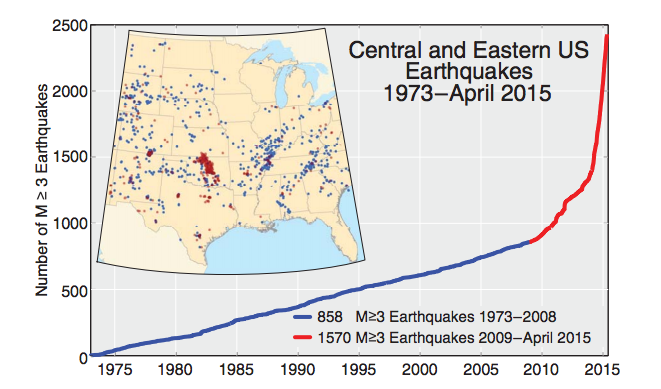
\includegraphics[width=0.7\textwidth]{induced}
   \caption{\label{inducedfig} From \cite{seis_induced}. Count of M $\geq3$ earthquakes in the central and eastern United States from 1973 to April 2015. Two abrupt increases in the earthquake rate occurred in 2009 and 2013. Red dots represent earthquakes that occurred between 2009 and April 2015, and blue dots represent earthquakes that occurred between 1973 and 2008. Prior to 2009, earthquakes were spread across the United States. Beginning in 2009 the earthquakes are tightly clustered in a few areas}. 
\end{wrapfigure}

The data used for enumerating this dimension of each well was the "Quaternary Fault and Fold Database of the United States," provided by the U.S. Geological Service. The data base included the shape and gepgraphical positioning of each fault in the U.S. as well as the slip rate, a measure of the activity of the fault. Following the same logic in (1) lead me to the formula 
$$score(n_i) =  \mathbb{E}\bigg[\sum_{j=0}^k \frac{s_j}{dist^2(n_i, r_j)}\bigg]$$
where $s_j$ here is the slip rate of the $j$th fault and $dist(n_i, r_j)$ is the distance between the $i$th injection site and the nearest point to it on the $j$th fault line. 


\item \emph{Proximity to and Size of Population Centers} 



The scoring for this dimension is based on data from the U.S. Census Beareu. Each of the 500 U.S. cities with the largest populations were listed with their populations and geographical coordinates. Similar logic was applied to scoring potential injection sites with respect to this dimension as was applied to the above dimension. However, in this instance we have $s_j$ as the total population of the $j$th city. This again gives,
$$score(n_i) =  \mathbb{E}\bigg[\sum_{j=0}^k \frac{s_j}{dist^2(n_i, r_j)}\bigg]$$


\item \emph{Proximity to National Parks}
\end{enumerate} 

Cover where you got your data and why you chose the features. dimensions you chose



\subsection{Fuzzy c-Means Clustering}\label{fuzz}.
So that this paper can be self contained, I include an introduction to Fuzzy c-Means clustering and related concepts. This section will consist of an introduction to clustering followed by the way in which it is applied to this work.

\subsubsection{Introduction to Fuzzy c-Means Clustering}


\subsubsection{Application of Fuzzy c-Means Clustering} 

\subsection{Analysis of Site Already in Use}
Talk about the few points that represent wells that are already in use and how they fit in your model. 


\section{Results}
These are some of the results

\begin{wrapfigure}{R}{0.5\textwidth}%this figure will be at the right
  \centering
  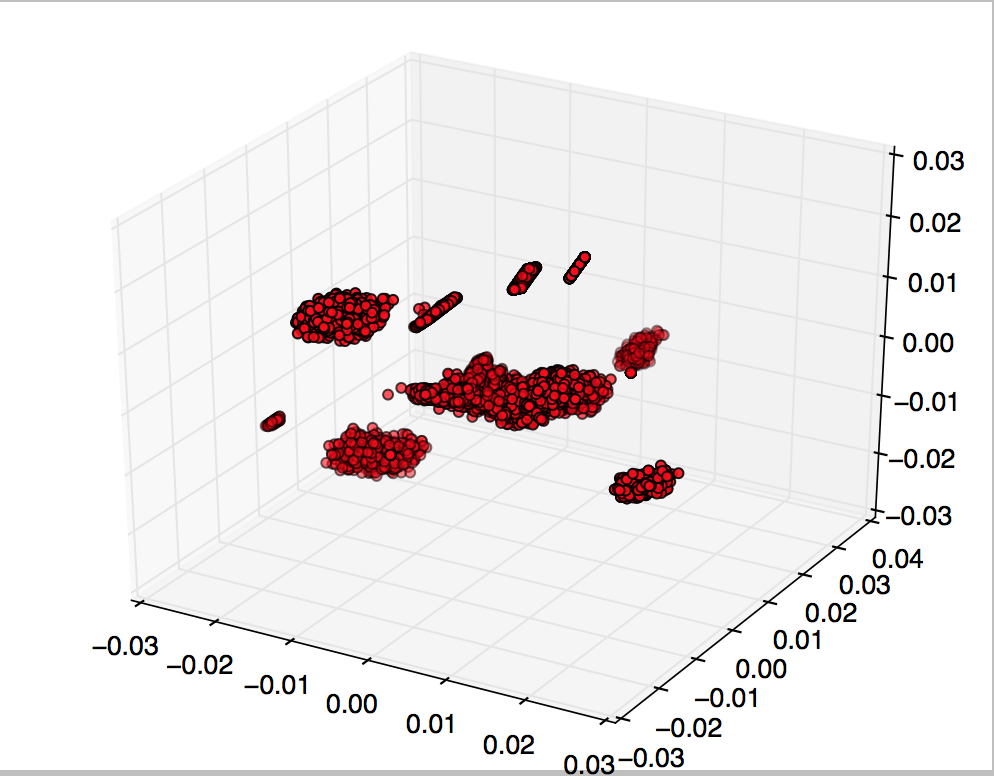
\includegraphics[width=0.5\textwidth]{clusters}
  \caption{\label{clusters} Results of the Fuzzy c-Means clustering on the data sample}. 
\end{wrapfigure}

\begin{wrapfigure}{L}{0.5\textwidth}%this figure will be at the right
   \centering
  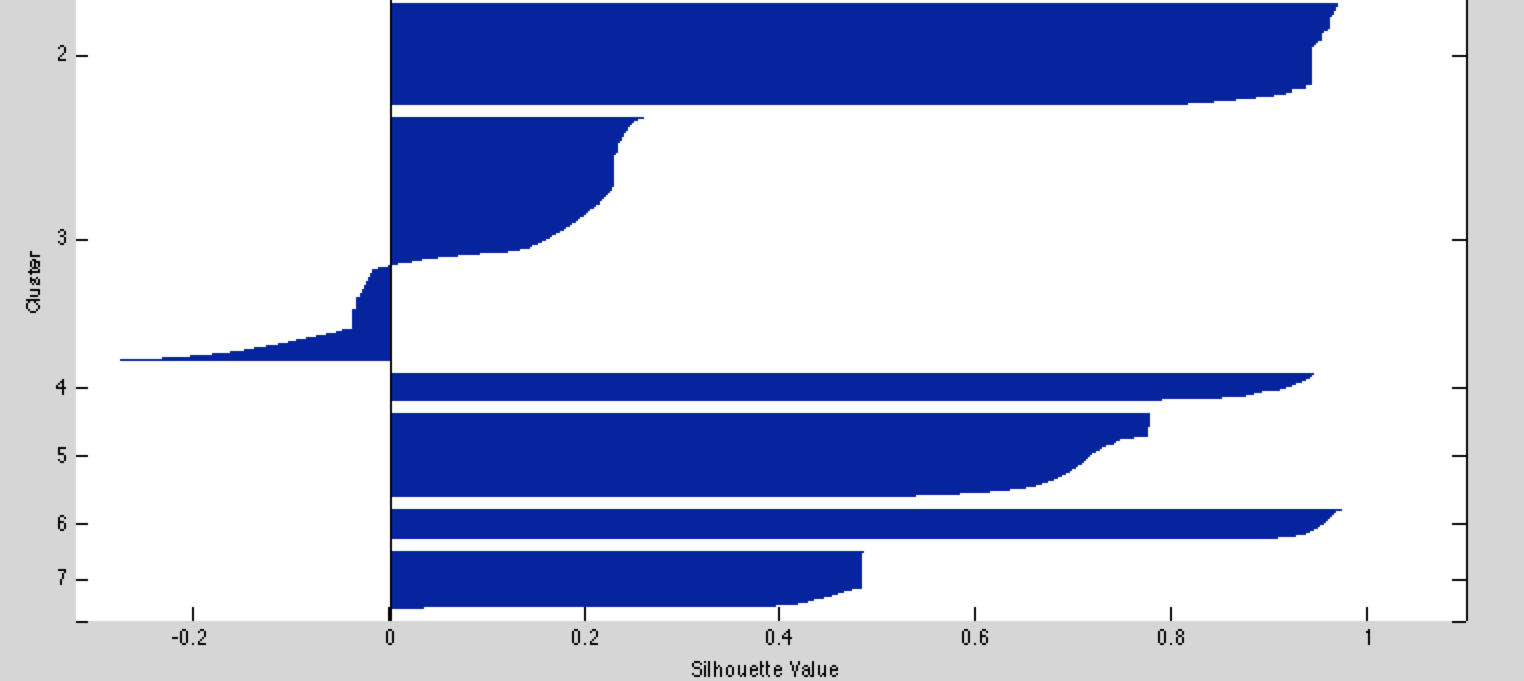
\includegraphics[width=0.5\textwidth]{k_means_sil}
   \caption{\label{k_means_sil} ... }. 
\end{wrapfigure}


\section{Discussion and Analysis}

\section{Future Work}
\subsection{Better Characterization of Saline Formations}
The 12 features isolated for characterization are a minimal set for reasonable characterization of saline formations. Better and more detailed (higher dimensional) characterizations of these formations would necessarily allow for more data for Fuzzy c-Means clustering to base its similarity measures on, thereby increasing the accuracy and effectiveness of this tool. Further dimensions include the existence of a caprock over the layer of porous rock. The existence of such a caprock is extremely important to the viability of a potential site as it plays an important part in keeping the injected carbon below the surface and in place.  

\subsection{Isolating Better Heuristics for Scoring Formation Dimensions}
\section{Conclusion}

 
\begin{thebibliography}{9}

\bibitem{QuantRiskS2014}
Wriedt, J., Deo, M., Han, W. S., and Lepinski, J.
\textit{A methodology for quantifying risk and likelihood of failure for carbon dioxide injection into deep saline reservoirs}
International Journal of Greenhouse Gas Control 20 (2014), 196-211.

\bibitem{midwestinject}
Albenze, Erik, and Sallie Greenberg. 
\textit{Midwest Geological Sequestration Consortium $\|$ Development Phase}
National Energy Technology Laboratory, 1 Nov. 2015. http://www.netl.doe.gov/publications/factsheets/project/NT42588.pdf.

\bibitem{midwestinject2}
McNemar, Andrea, and Neeraj Gupta. 
\textit{Midwest Regional Carbon Sequestration Partnership $\|$ Development Phase}
National Energy Technology Laboratory, 1 Nov. 2015. http://www.netl.doe.gov/publications/factsheets/project/NT42589.pdf.

\bibitem{southeastinject}
Brown, Bruce, and Ken Nemeth. 
\textit{Southeast Regional Carbon Sequestration Partnership $\|$ Validation Phase}
National Energy Technology Laboratory, 1 Dec. 2012. http://www.netl.doe.gov/publications/factsheets/project/NT42590-P2.pdf.

\bibitem{whysaline}
\textit{Carbon Storage R\&D} Department of Energy. Office of Fossil Energy. Web. 01 May 2016.

\bibitem{atlas}
Friedmann, S. 
\textit{Carbon Storage Atlas V} 
National Energy Technology Laboratory, 1 Aug 2015.

\bibitem{natcarb_risk}
\textit{Carbon Storage Technology Program Plan}
Clean Coal Research Program, Department of Energy. Office of Fossil Energy. 1 Dec. 2014.

\bibitem{seis_induced}
Rubinstein, Justin L., Mahani, Alireza B.
\textit{Myths and Facts on Wastewater Injection, Hydraulic Fracturing, Enhanced Oil Recovery, and Induced Seismicity}
Seismological Research Letters 86, 4 (2015), 1-8. 

\bibitem{PredRisk2013}
Balashov, Victor N., et al.
\textit{Predictive modeling of CO 2 sequestration in deep saline sandstone reservoirs: impacts of geochemical kinetics}
Applied geochemistry 30 (2013): 41-56.

\end{thebibliography}
\end{document}
